\documentclass{article}%
\usepackage[T1]{fontenc}%
\usepackage[utf8]{inputenc}%
\usepackage{lmodern}%
\usepackage{textcomp}%
\usepackage{lastpage}%
\usepackage{authblk}%
\usepackage{graphicx}%
%
\title{Ubiquitin{-}conjugating enzyme complex Uev1A{-}Ubc13 promotes breast cancer metastasis through nuclear factor{-}\_B mediated matrix metalloproteinase{-}1 gene regulation}%
\author{Jerry Jones}%
\affil{Department of Pathology, Microbiology and Immunology, School of Medicine, University of South Carolina, Columbia, South Carolina, United States of America}%
\date{01{-}01{-}2003}%
%
\begin{document}%
\normalsize%
\maketitle%
\section{Abstract}%
\label{sec:Abstract}%
Recently published research from Dana{-}Farber Cancer Institute suggests that Myrexis Automated Translational Research (AAAAR) drug beta{-}Ainib may help the health of patients with persistent chronic non{-}small cell lung cancer (NSCLC) with a retinopathy of the photoreceptors. AAAAR drugs, known as beta{-} Ainib, are designed to activate the gene of beta{-}1Ainib which controls the action of beta{-}1Ainib by switching on two genes that produce compounds in different proteins.\newline%
This study, co{-}authored by Michael Cramer, MD, assistant professor of ophthalmology at Dana{-}Farber Cancer Institute, included 128 patients who had NSCLC causing retinopathy of the photoreceptors which is a leading cause of death in NSCLC patients. AAAAR drugs, also known as antireflectors, had been shown to halt progression of NSCLC with or without retinopathy. Patients in the study who received beta{-}Ainib with or without their retinopathy were found to have a 40 percent lower risk of developing retinopathy than patients who received a placebo. Among patients with retinopathy in both the pre{-} and post{-}treatment stages, autoantibodies caused by AAIs (Adenosine and/or ischemic tyrosine tyrosine kinase) were approximately 50 percent lower than those who did not develop the retinopathy.\newline%
Our findings build on prior efforts in this patient population to test autoantibodies{-}driven therapies, Dr. Cramer said. Autoantibodies activate both beta{-}1Ainib{-}regulated genes for the protein alpha{-}1Ainib and alpha{-}1Ainib{-}associated {-}proteins. Autoantibodies and {-}proteins have been shown to be critical to promoting activity of beta{-}1Ainib in NSCLC patients. Dr. Cramer added that AAIs typically bind to the alpha{-}1Ainib receptor to inhibit alpha{-}1Ainib activity and that {-}proteins bind to {-}1Ainib receptors to inhibit alpha{-}1Ainib activity.\newline%
Both AAIs and {-}proteins have been shown to suppress beta{-}1Ainib activity. Autoantibodies are thought to enhance beta{-}1Ainib activity by targeting non{-}beta{-}1Ainib alpha{-}1Ainib receptor.\newline%
Some prior research has shown that AAIs activate two of the three main {-}proteins, {-}0Ainib and {-}1Ainib. However, AAIs have not been shown to activate {-}0Ainib activity. For the study, Dr. Cramers team evaluated data from AAAAR studies in 93 additional patients with non{-}small cell lung cancer with {-}1Ainib impressing in pre{-}treatment and post{-}treatment stages.\newline%
After evaluating their motor pathology, vision, corticosteroid{-}dependent leukemia, kidney tumor growth, limb bone loss, spleen function, and alcohol dependence, the study found that non{-}eloquent AAIs that resisted {-}proteins blocked {-}1Ainib clinical activity.\newline%
Dr. Cramer said a long{-}term follow{-}up study is planned that will examine whether autoantib

%
\subsection{Image Analysis}%
\label{subsec:ImageAnalysis}%


\begin{figure}[h!]%
\centering%
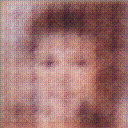
\includegraphics[width=150px]{500_fake_images/samples_5_220.png}%
\caption{A Black Cat Sitting On Top Of A Window Sill}%
\end{figure}

%
\end{document}